%\addcontentsline{toc}{chapter}{Development Process}
\chapter{Design} % You should concentrate on the more important aspects of the design. It is essential that an overview is presented before going into detail. As well as describing the design adopted it must also explain what other designs were considered and why they were rejected.The design should describe what you expected to do, and might also explain areas that you had to revise after some investigation.Typically, for an object-oriented design, the discussion will focus on the choice of objects and classes and the allocation of methods to classes. The use made of reusable components should be described and their source referenced. Particularly important decisions concerning data structures usually affect the architecture of a system and so should be described here.How much material you include on detailed design and implementation will depend very much on the nature of the project. It should not be padded out. Think about the significant aspects of your system. For example, describe the design of the user interface if it is a critical aspect of your system, or provide detail about methods and data structures that are not trivial. Do not spend time on long lists of trivial items and repetitive descriptions. If in doubt about what is appropriate, speak to your supervisor. You should also identify any support tools that you used. You should discuss your choice of implementation tools - programming language, compilers, database management system, program development environment, etc.Some example sub-sections may be as follows, but the specific sections are for you to define.

@TODO - leading up to the Design section of the report, we should already have established:

* background \& objectives
* requirements
* the switch to an agile approach, encompassing design, development and testing all at once.

% ---

As has already been discussed, I opted for a hybrid approach of a plan-driven methodology to begin with, followed by an agile approach for the implementation. The design stage is where one methodology merges into the other.

I invested a lot of time in clarifying requirements, so that I could establish common classes and methods and processes that can be reused, which would have an effect on my design.

I felt that certain design documentation, such as a database schema, would be worth spending time creating and could be designed up front. Other things, such as class diagrams would not be suitable to be designed upfront, since I'd be refactoring my code throughout the process and it would fall out of line with the documentation.

\section{Overall Architecture}

My project can be broken down into three main components:

\begin{enumerate}
    \item \textbf{Core platform}, AKA SmartResolution. This is the ODR software that I spent the majority of my time developing.
    
    \item \textbf{Maritime collision module}. This is a plugin for the SmartResolution software that defines a "Maritime Collision" dispute type and offers custom actions and business logic for these specialised cases.
    
    \item \textbf{SmartResolution Marketplace}, AKA smartresolution.org. 
\end{enumerate}

When I considered the commercial viability of the software (see appendix~\ref{appendix:commercialViability}), I drew a parallel with the blogging software WordPress. My overall architecture follows the same principle as theirs:

\begin{enumerate}
    \item \textbf{WordPress platform}: blogging software that can be downloaded, installed and hosted on your own server.
    
    \item \textbf{WordPress plugin}: a self-contained package that can be installed to a WordPress installation and augment the core installation with additional functionality.
    
    \item \textbf{Plugin Directory}: a searchable area of the WordPress.org website, accessible directly through your own WordPress installation, allowing the painless and automatic installation of plugins. % https://wordpress.org/plugins/
\end{enumerate}

\subsection{Core platform}

SmartResolution [REF] is the ODR platform offering the core online dispute resolution requirements, such as organisation and user registration, dispute creation, messaging, file uploads, and so on. It offers the minimum facilities necessary to successfully negotiate a dispute online.

As it is the basis of all the other components, it is also the most thoroughly engineered and is backed up with integration and unit tests, continuous integration, automated code quality checks and dependency status checks.

\subsection{Maritime collision module}

This module is separate from the core platform and lives in its own repository [REF]. It can be installed to any SmartResolution installation by being deployed to the top-level "modules" directory; no further configuration is required.

As discussed in the background and initial requirements, it was intended for this to be a feature-rich module that could find similar historic cases, cross-check agents' answers with maritime law, and approximate the likelihood of an agent's success in court. This is still theoretically possible. However, given the lack of time and resources, I've had to create this as more of a prototype; a teasing glimpse as to what might be possible given a few more development hours.

\subsection{SmartResolution Marketplace}

This is the vendor site for SmartResolution, explaining what SmartResolution is and offering a download link to a production-ready version. Its subdomain, demo.smartresolution.org, has a live demo of the SmartResolution software installed so that users can try out the software before they download. However, the main purpose for smartresolution.org is the \emph{Marketplace} facility.

This facility, like WordPress' "Plugin Directory", is tightly coupled to the administrative functions in the core software. Administrators are able to browse, download and install SmartResolution modules from smartresolution.org, from within the SmartResolution installation itself.

\section{SmartResolution design}

As the basis of all of the other components, SmartResolution itself required the most design preparation.

\subsection{SmartResolution directory structure}

\dirtree{%
.1 data.
.1 deploy.
.1 features.
.1 modules.
.1 test.
.1 vendor.
.1 webapp.
.2 controller.
.2 model.
.2 view.
.2 index.php.
.2 routes.php.
.1 .travis.yml.
.1 composer.json.
.1 Gemfile.
}

\lstinline{data} contains fixture data for tests. This is also where the test and production SQLite3 databases reside.

\lstinline{deploy} contains an installation script to ease setup for new SmartResolution installations, as well as a bundled server to make it easier for developers to verify that the software is installed correctly.

\lstinline{features} contains my Cucumber features and Ruby step definitions.

\lstinline{modules} contains any installed SmartResolution modules. This is where the maritime collision module resides.

\lstinline{test} contains my PHP unit tests.

\lstinline{vendor} is an automatically generated directory, created by Composer, containing all of SmartResolution's dependencies.

\lstinline{webapp} contains the core ODR platform, which uses an MVCR compound design pattern (\lstinline{routes.php} defines the routing component).

Finally, at the top level we have a few interesting files:

\lstinline{.travis.yml} - an instructions file for Travis Continuous Integration, describing how to set up the project and run its tests. The same commands are required in the one-step installation script (\lstinline{deploy/install.php}), so I use PHP to parse the YAML in this Travis configuration file to avoid duplication.

\lstinline{composer.json} - describes SmartResolution's dependencies. Developers can install all dependencies simply by running \lstinline{\$ composer install}.

\lstinline{Gemfile} - describes SmartResolution's Ruby dependencies. Required for the Cucumber and Ruby integration tests.

\subsection{Database schema}

\begin{figure}[h!]
  \centering
    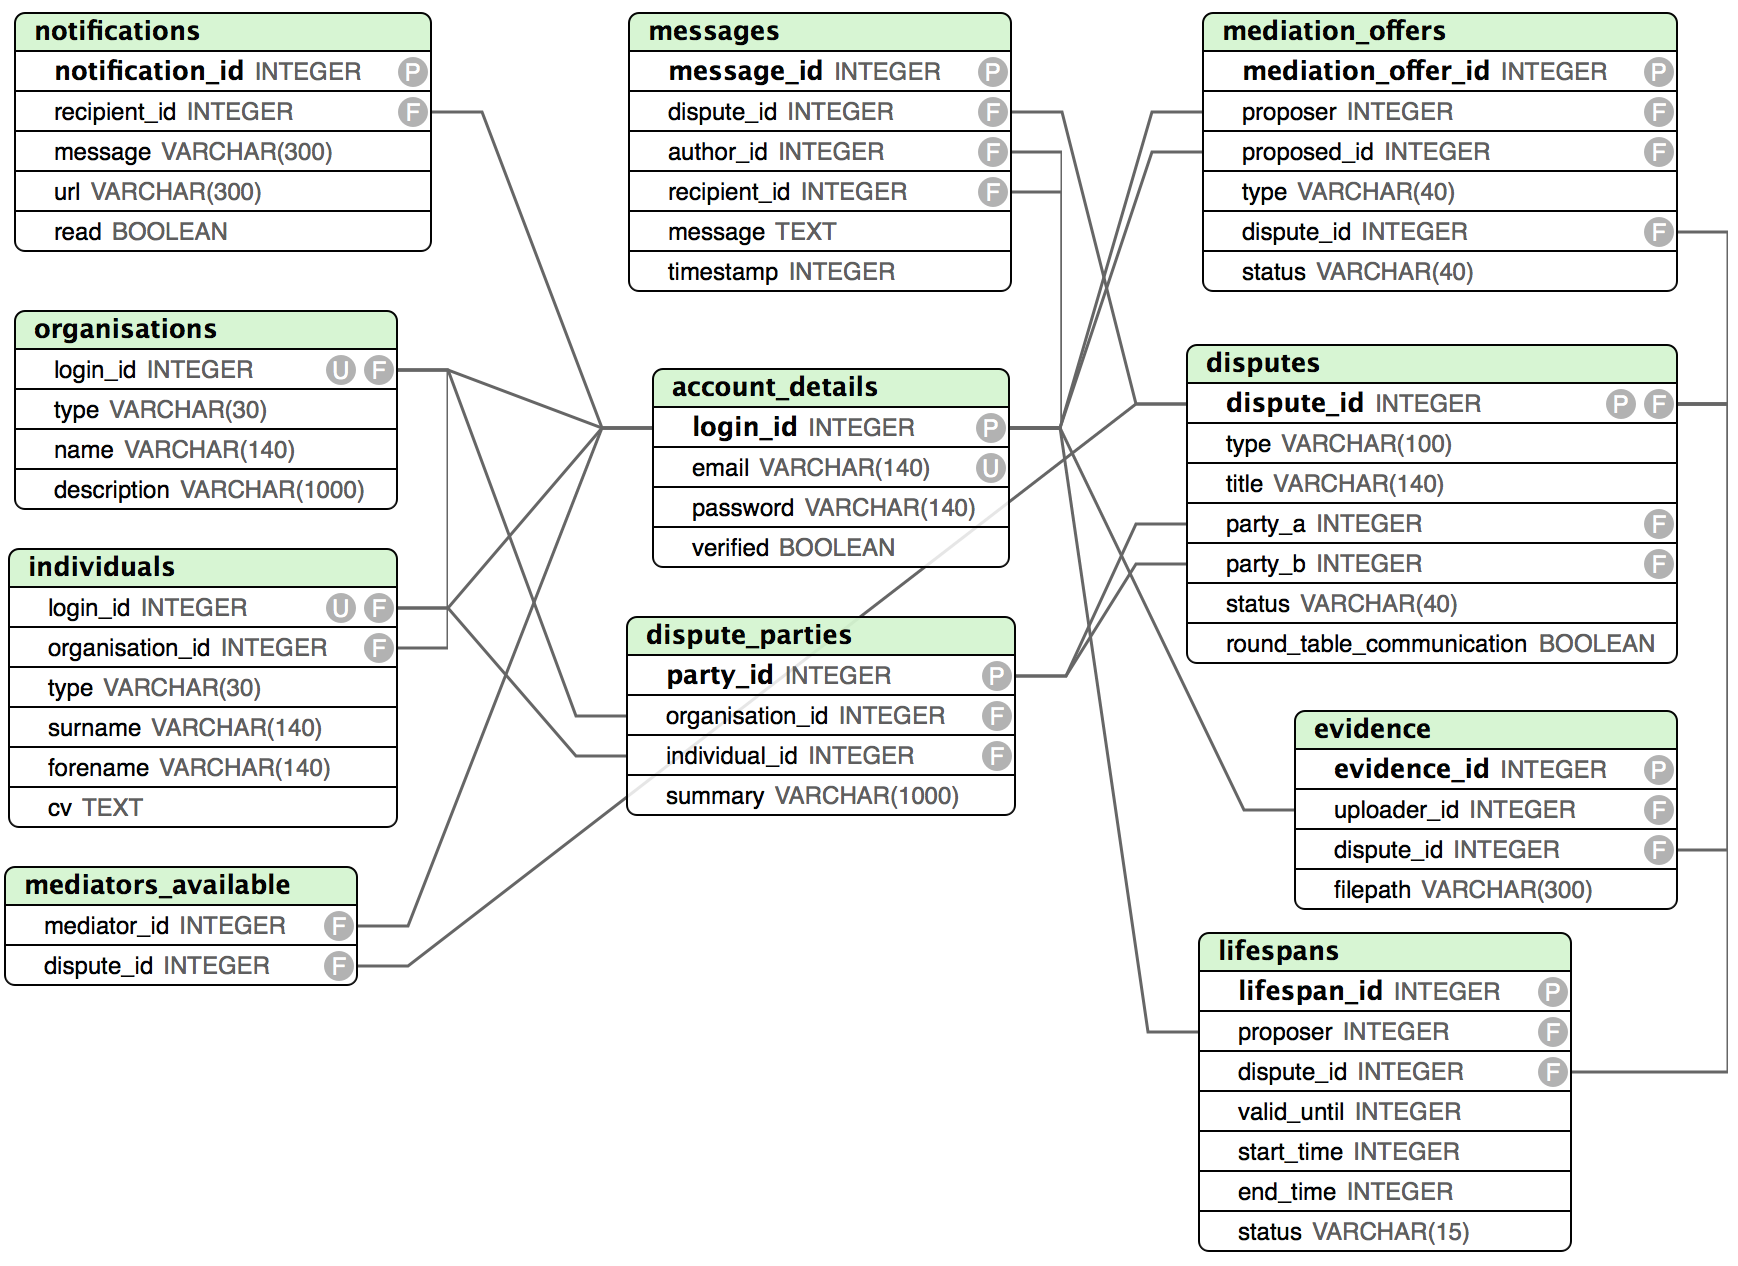
\includegraphics[width=\textwidth]{database}
  \caption{Database schema for the SmartResolution core platform}
  \label{uml:databaseSchema}
\end{figure}

Figure~\ref{uml:databaseSchema} shows the database schema for the SmartResolution core platform, generated directly from \lstinline{data/db.sql} using SQLEditor, for the purposes of this report.

\lstinline{P} symbols refer to primary keys, \lstinline{F} symbols refer to foreign keys, and \lstinline{U} symbols refer to unique integrity constraints. Lines generally denote where one table key references another, i.e. a foreign key visualisation.

For a full explanation and justification of the database design, please refer to appendix~\ref{appendix:database}.

\section{User Interface}

\section{Other relevant sections}